%! Author = denis
%! Date = 20/08/2026

\begin{frame}{Contagem e controle: máquinas de estado}
    \small
    \begin{block}{Definição}
        Uma máquina de estados é um circuito sequencial que muda de
        comportamento conforme seu estado atual e os eventos de entrada.
    \end{block}

    \centering
    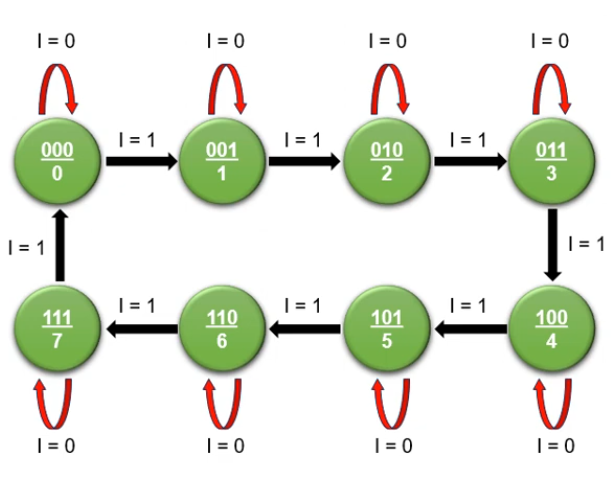
\includegraphics[
        width=\linewidth,
        height=0.65\textheight,
        keepaspectratio
    ]{images/maquina_de_estado.png}
    
\end{frame}